\documentclass{article}%
\usepackage[T1]{fontenc}%
\usepackage[utf8]{inputenc}%
\usepackage{lmodern}%
\usepackage{textcomp}%
\usepackage{lastpage}%
\usepackage{geometry}%
\geometry{margin=0.7in}%
\usepackage{ragged2e}%
\usepackage{graphicx}%
\usepackage{fancyhdr}%
%
\fancypagestyle{header}{%
\renewcommand{\headrulewidth}{0pt}%
\renewcommand{\footrulewidth}{0pt}%
\fancyhead{%
}%
\fancyfoot{%
}%
\fancyhead[L]{%
Page date: %
\linebreak%
2023{-}02{-}04%
}%
\fancyhead[C]{%
Georgia Institute of Technology%
}%
\fancyhead[R]{%
Page \thepage\ of \pageref{LastPage}%
}%
}%
%
\begin{document}%
\normalsize%
\pagestyle{header}%
\begin{minipage}{\textwidth}%
\centering%
\begin{Large}%
\textbf{HW2: Problem 3}%
\end{Large}%
\linebreak%
\begin{large}%
\textbf{Ian Dover}%
\end{large}%
\end{minipage}%
\section{Read and display the image:}%
\label{sec:Readanddisplaytheimage}%
The rose on ice image:%


\begin{figure}[h!]%
\centering%
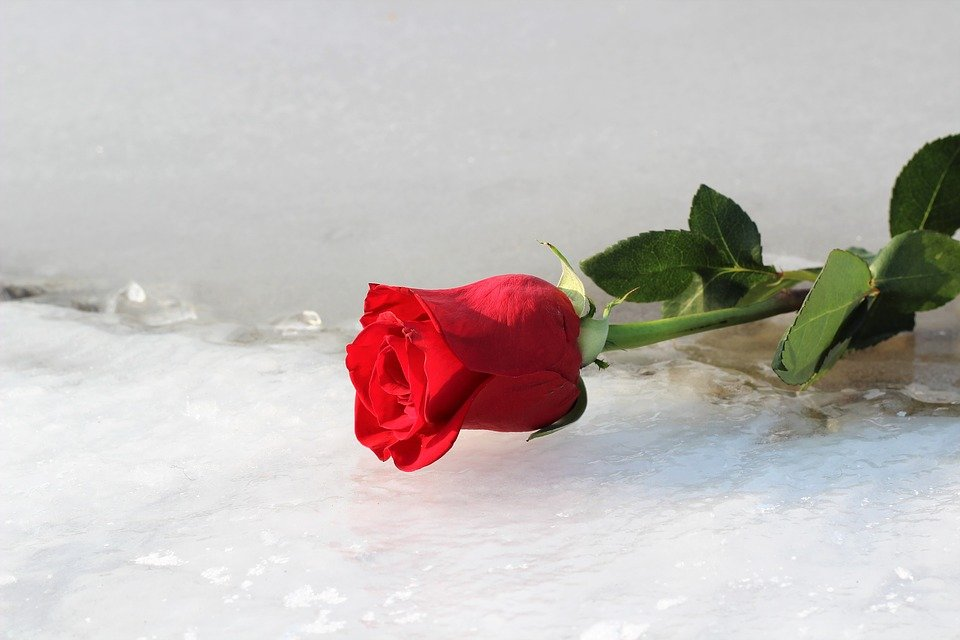
\includegraphics[width=120px]{/com.docker.devenvironments.code/reports/problem3/../../images/RoseonIce-1.jpg}%
\caption{Rose on ice image.}%
\end{figure}

%
\section{Part 1}%
\label{sec:Part1}%
\subsection{K{-}means Clustering: 2 Clusters}%
\label{subsec:K{-}meansClustering2Clusters}%
Image split into two clusters:%


\begin{figure}[h!]%
\centering%
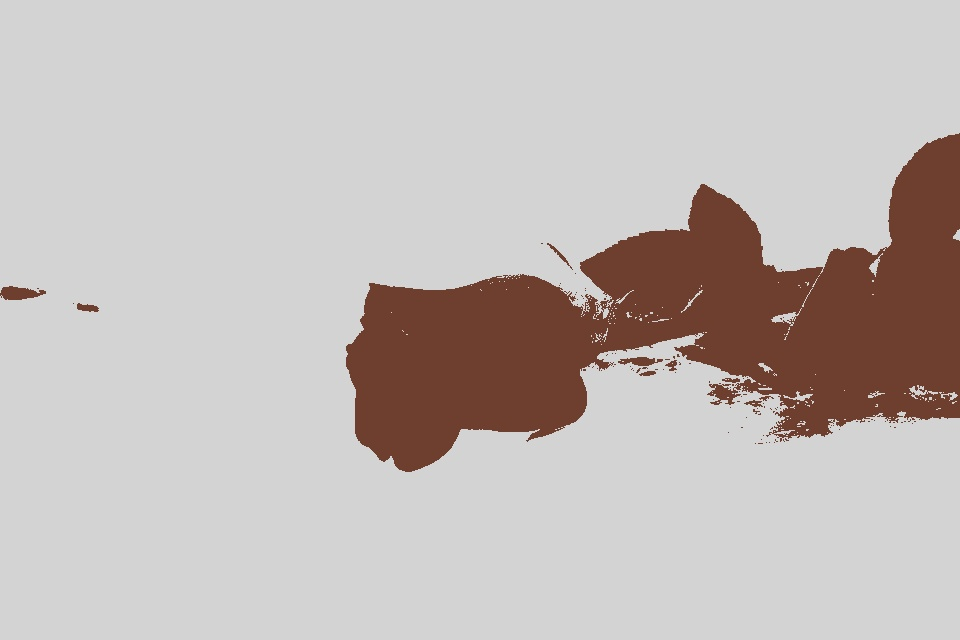
\includegraphics[width=120px]{/com.docker.devenvironments.code/reports/problem3/../../output/problem3/p3_1_kmeans_2.jpg}%
\caption{Image with K{-}means Clustering: 2 Clusters.}%
\end{figure}

%
\subsection{K{-}means Clustering Histogram: 2 Clusters}%
\label{subsec:K{-}meansClusteringHistogram2Clusters}%
Histogram of the image split into two clusters:%


\begin{figure}[h!]%
\centering%
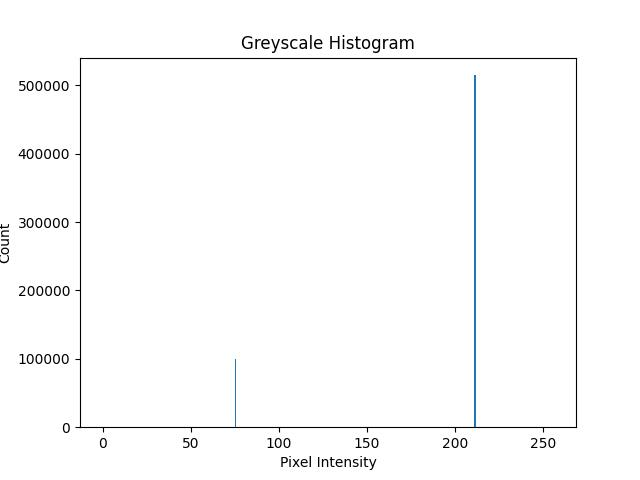
\includegraphics[width=200px]{/com.docker.devenvironments.code/reports/problem3/../../output/problem3/p3_1_kmeans_2_histogram.jpg}%
\caption{Histogram of image with K{-}means Clustering: 2 Clusters.}%
\end{figure}

%
\newpage%
\subsection{K{-}means Clustering: 3 Clusters}%
\label{subsec:K{-}meansClustering3Clusters}%
Image split into three clusters:%


\begin{figure}[h!]%
\centering%
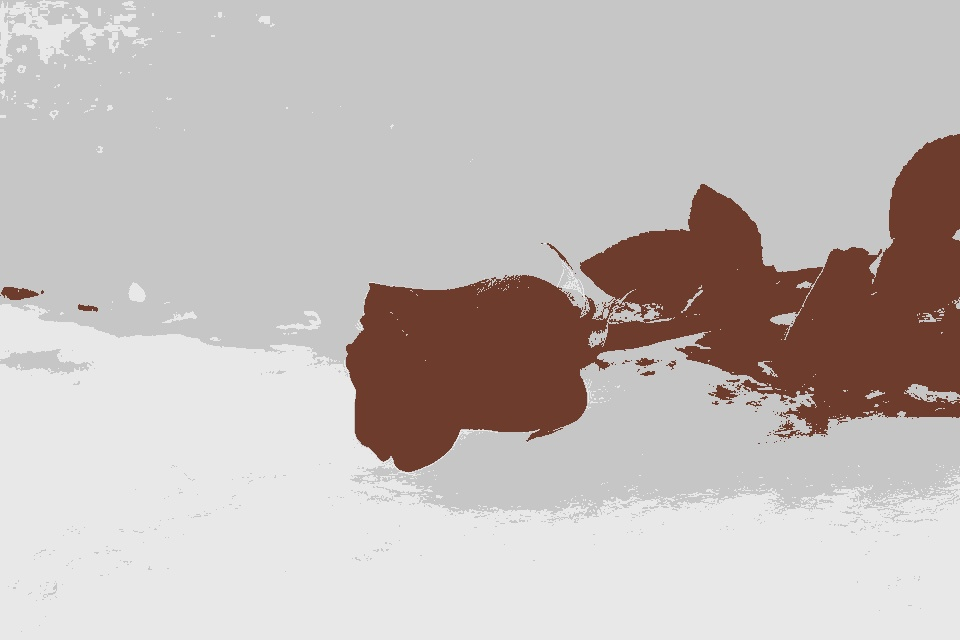
\includegraphics[width=120px]{/com.docker.devenvironments.code/reports/problem3/../../output/problem3/p3_1_kmeans_3.jpg}%
\caption{Image with K{-}means Clustering: 3 Clusters.}%
\end{figure}

%
\subsection{K{-}means Clustering Histogram: 3 Clusters}%
\label{subsec:K{-}meansClusteringHistogram3Clusters}%
Histogram of the image split into three clusters:%


\begin{figure}[h!]%
\centering%
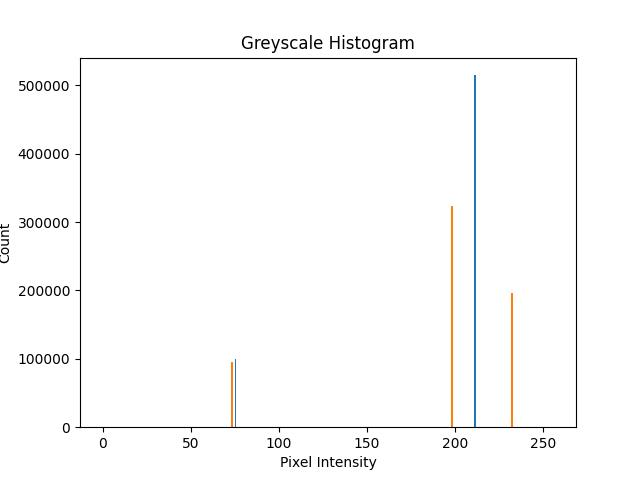
\includegraphics[width=200px]{/com.docker.devenvironments.code/reports/problem3/../../output/problem3/p3_1_kmeans_3_histogram.jpg}%
\caption{Histogram of image with K{-}means Clustering: 3 Clusters.}%
\end{figure}

%
\subsection{K{-}means Clustering: 4 Clusters}%
\label{subsec:K{-}meansClustering4Clusters}%
Image split into four clusters:%


\begin{figure}[h!]%
\centering%
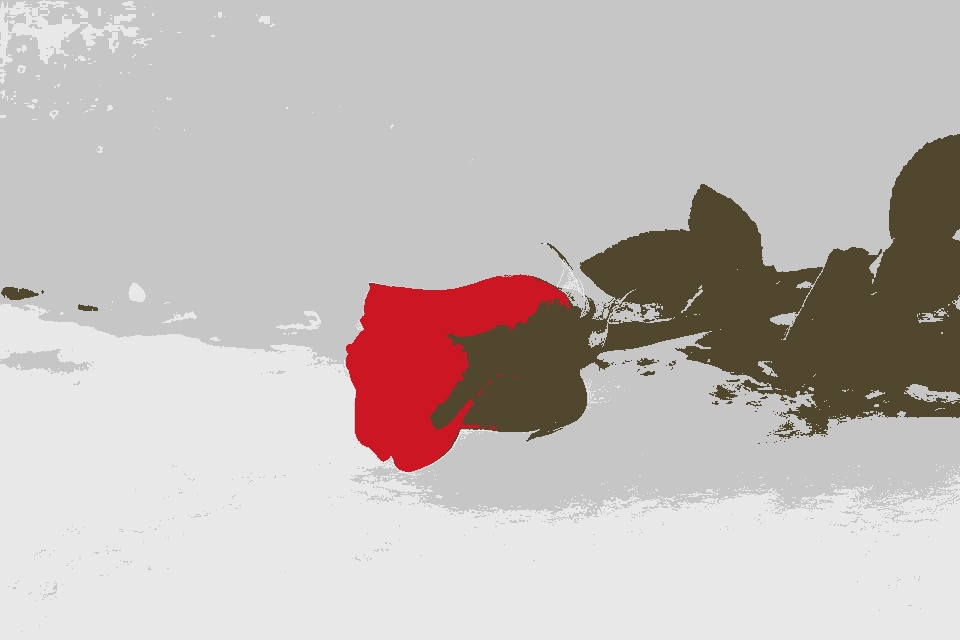
\includegraphics[width=120px]{/com.docker.devenvironments.code/reports/problem3/../../output/problem3/p3_1_kmeans_4.jpg}%
\caption{Image with K{-}means Clustering: 4 Clusters.}%
\end{figure}

%
\newpage%
\subsection{K{-}means Clustering Histogram: 4 Clusters}%
\label{subsec:K{-}meansClusteringHistogram4Clusters}%
Histogram of the image split into four clusters:%


\begin{figure}[h!]%
\centering%
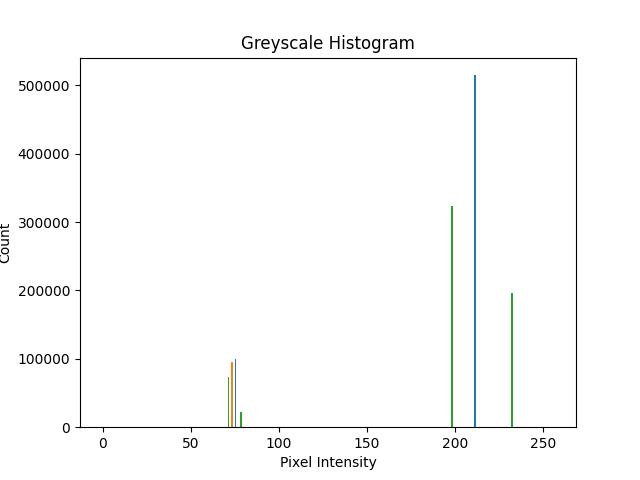
\includegraphics[width=200px]{/com.docker.devenvironments.code/reports/problem3/../../output/problem3/p3_1_kmeans_4_histogram.jpg}%
\caption{Histogram of image with K{-}means Clustering: 4 Clusters.}%
\end{figure}

%
\subsection{K{-}means Clustering: 5 Clusters}%
\label{subsec:K{-}meansClustering5Clusters}%
Image split into five clusters:%


\begin{figure}[h!]%
\centering%
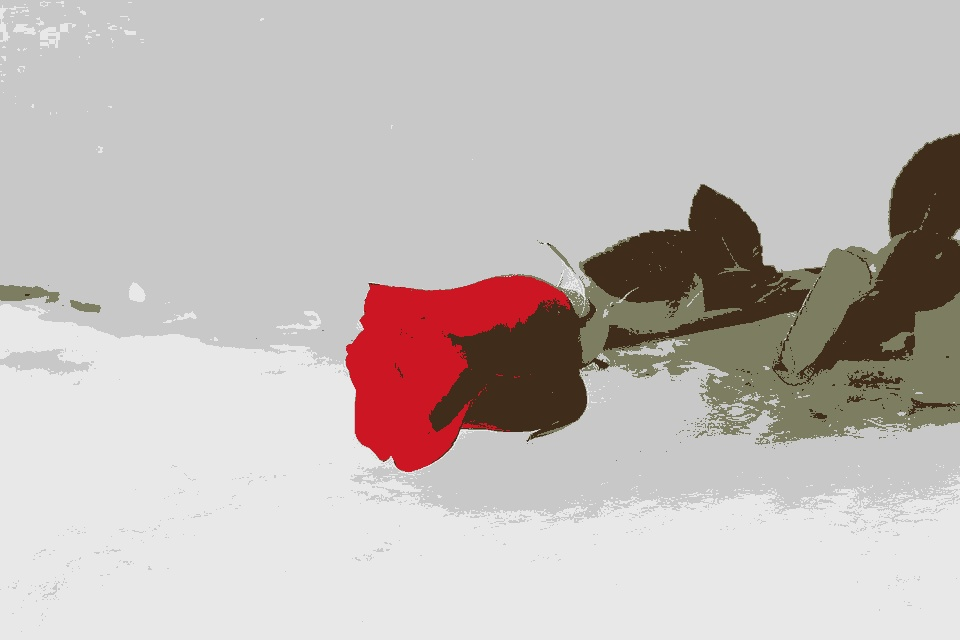
\includegraphics[width=120px]{/com.docker.devenvironments.code/reports/problem3/../../output/problem3/p3_1_kmeans_5.jpg}%
\caption{Image with K{-}means Clustering: 5 Clusters.}%
\end{figure}

%
\subsection{K{-}means Clustering Histogram: 5 Clusters}%
\label{subsec:K{-}meansClusteringHistogram5Clusters}%
Histogram of the image split into five clusters:%


\begin{figure}[h!]%
\centering%
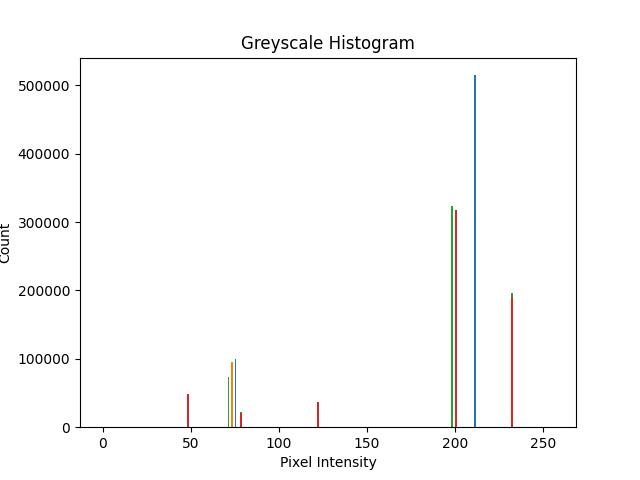
\includegraphics[width=200px]{/com.docker.devenvironments.code/reports/problem3/../../output/problem3/p3_1_kmeans_5_histogram.jpg}%
\caption{Histogram of image with K{-}means Clustering: 5 Clusters.}%
\end{figure}

%
\section{Part 2}%
\label{sec:Part2}%
\subsection{Convert the image into greyscale:}%
\label{subsec:Converttheimageintogreyscale}%


\begin{figure}[h!]%
\centering%
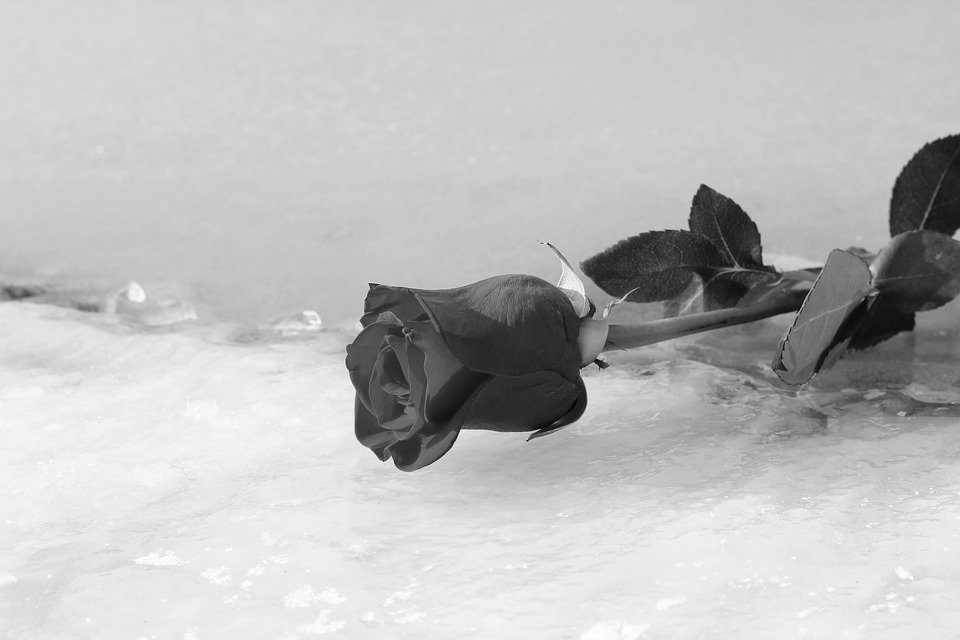
\includegraphics[width=120px]{/com.docker.devenvironments.code/reports/problem3/../../output/problem3/p3_2_grayscale.jpg}%
\caption{Convert the image into greyscale.}%
\end{figure}

%
\subsection{Plot the histogram:}%
\label{subsec:Plotthehistogram}%


\begin{figure}[h!]%
\centering%
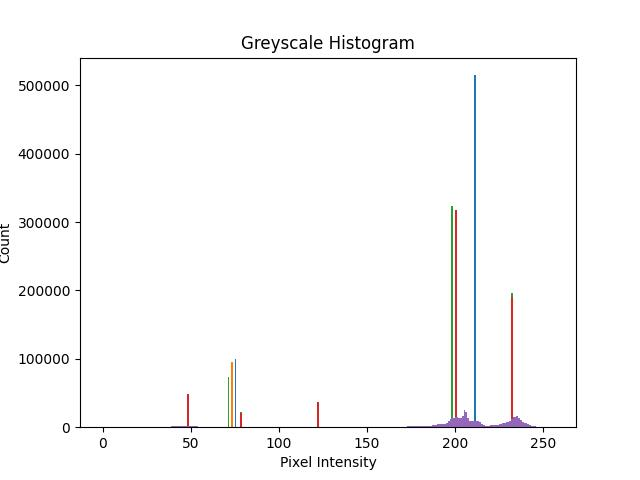
\includegraphics[width=200px]{/com.docker.devenvironments.code/reports/problem3/../../output/problem3/p3_2_histogram.jpg}%
\caption{Histogram of greyscale image.}%
\end{figure}

%
\section{Part 3}%
\label{sec:Part3}%
\subsection{Image thresholded using Otsu's method.}%
\label{subsec:ImagethresholdedusingOtsusmethod.}%
The optimal threshold for the grayscale image determined by Otsu is: 143%


\begin{figure}[h!]%
\centering%
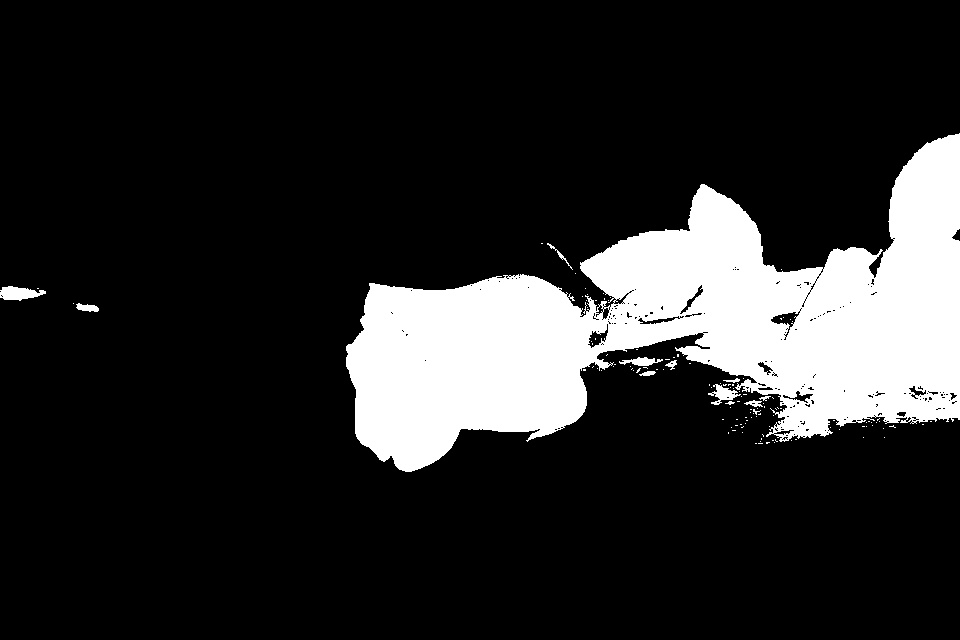
\includegraphics[width=120px]{/com.docker.devenvironments.code/reports/problem3/../../output/problem3/p3_3_otsu_threshold_image.jpg}%
\caption{Image thresholded using Otsu's method.}%
\end{figure}

%
\subsection{Plot the histogram of the image that underwent Otsu thresholding:}%
\label{subsec:PlotthehistogramoftheimagethatunderwentOtsuthresholding}%


\begin{figure}[h!]%
\centering%
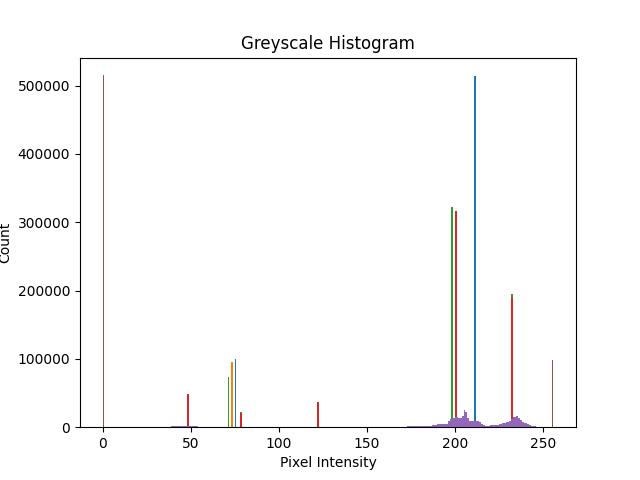
\includegraphics[width=200px]{/com.docker.devenvironments.code/reports/problem3/../../output/problem3/p3_3_otsu_histogram.jpg}%
\caption{Histogram of greyscale image.}%
\end{figure}

%
\end{document}